\documentclass{beamer}
\usetheme{Madrid}
\usepackage{amsmath}
\usepackage{graphicx}
\usepackage{mathrsfs}
\usepackage{tikz}
\usepackage{color}
\usetikzlibrary{bayesnet}
\newcommand*\diff{\mathop{}\!\mathrm{d}}
\newcommand*\Diff[1]{\mathop{}\!\mathrm{d^#1}}
\title{Nonparameteric Learning}
\author{Jie Tang}

\begin{document}


\begin{frame}
\titlepage
\end{frame}

\begin{frame}
\frametitle{Outline}
\tableofcontents[pausesections]
\end{frame}

\section{Kernels}
\section{Gaussian Process}


\section{Dirichlet Process}

\subsection{Gaussian Mixture}
\begin{frame}
	\frametitle{Motivating Example}
	\begin{itemize}
		\item We're give a data set which are generated by a mixture of Gaussian.
		\item How to model the data and cluster them?
	\end{itemize}
	\centering
	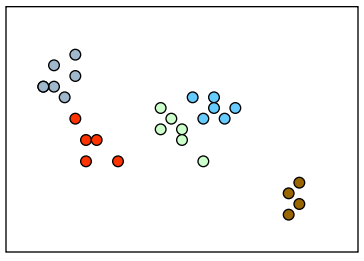
\includegraphics[width=0.6\textwidth]{img/motive.png}
\end{frame}

\begin{frame}
\frametitle{Gaussian Mixture Clustering}

\begin{columns}
\column{0.6\textwidth}
\begin{itemize}

	\item Suppose the dataset is generated by $K$ Gaussian components 
	\item Generating process:
\begin{align*}
\phi_k = (\mu_k, \Sigma_k) & \sim \mathcal{NIW}(\nu) \\
\pi & \sim \text{Dirichlet}(\alpha/K, \ldots, \alpha/K) \\
z_i & \sim \text{Multinomial}(\pi) \\
x_i & \sim \mathcal{N}(\mu_{z_i}, \Sigma_{z_i})
\end{align*}
where 
\begin{align*}
\mathcal{NIW}(\nu) & : \text{conjugate prior of Gaussian} \\
Dirichlet(\ldots) & : \text{conjugate prior of multinomial} \\
z_i & : \text{mixture indicator of } x_i
\end{align*}
\end{itemize}
\column{0.4\textwidth}
\centering
      \tikz{ %
        
        \node[const] (alpha) {$\alpha$} ;
        \node[latent, below=of alpha] (pi) {$\pi$} ; 
        \node[latent, below=of pi] (z) {$z_i$} ;
        \node[obs, below=of z] (x) {$x_i$} ;        

        
        \node[latent, right=of z] (phi) {$\phi_k$} ; %
        \node[const, above=of phi] (nu) {$\nu$} ; %

        \edge{nu}{phi} ;
        \edge{alpha}{pi} ;
        \edge{pi}{z} ;
        \edge{z}{x} ;
        \edge{phi}{x} ;
        \plate[inner sep=0.25cm, xshift=-0.12cm, yshift=0.12cm]{plate1}{(z)(x)}{$i$} ;
        \plate[inner sep=0.25cm, xshift=-0.12cm, yshift=0.12cm]{plate2}{(phi)}{$k$} ;
      }
\end{columns}
\end{frame}

\begin{frame}
	\frametitle{How to choose K?}
	\begin{itemize}
		\item How many clusters?
		\begin{center}
			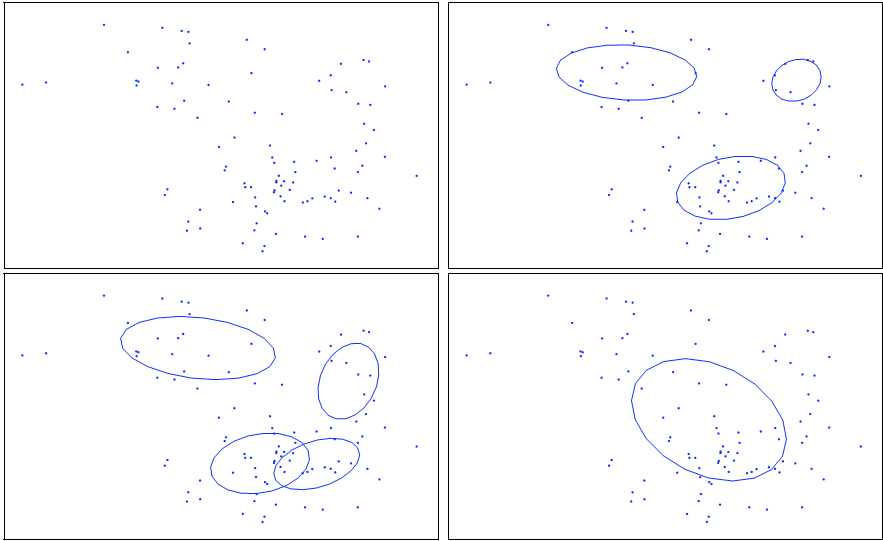
\includegraphics[width=0.6\textwidth]{img/unknown.png}
		\end{center}		
		\item What if let $K \rightarrow \infty$?
	\end{itemize}
\end{frame}

\begin{frame}
	\frametitle{Infinity Mixture Models}	
\begin{columns}
	\column{0.6\textwidth}
	\begin{itemize}
		\item Imagine $K\gg 0$, 
		\item In Bayesian inference, we integrate $\phi_k$ and $\pi$ out. Number of latent variables doesn't grow with $K$ -- No overfitting
		\item At most $n$ {\em active} components are associated with data
		\item It's an {\em infinite mixture model}
		\item Issue: can we take $K \rightarrow \infty$? What's the limiting model?
	\end{itemize}
	\column{0.4\textwidth}
	\centering
	\tikz{ %
		
		\node[const] (alpha) {$\alpha$} ;
		\node[latent, below=of alpha] (pi) {$\pi$} ; 
		\node[latent, below=of pi] (z) {$z_i$} ;
		\node[obs, below=of z] (x) {$x_i$} ;        
		
		
		\node[latent, right=of z] (phi) {$\phi_k$} ; %
		\node[const, above=of phi] (nu) {$\nu$} ; %
		
		\edge{nu}{phi} ;
		\edge{alpha}{pi} ;
		\edge{pi}{z} ;
		\edge{z}{x} ;
		\edge{phi}{x} ;
		\plate[inner sep=0.25cm, xshift=-0.12cm, yshift=0.12cm]{plate1}{(z)(x)}{$i$} ;
		\plate[inner sep=0.25cm, xshift=-0.12cm, yshift=0.12cm]{plate2}{(phi)}{$\infty$} ;
	}
\end{columns}
\end{frame}

\begin{frame}
	\frametitle{An Alternative View of Gaussian Mixture}
	
	\begin{columns}
		\column{0.7\textwidth}
		\begin{itemize}
			\item	Mixture paramtere for each data point can be sampled directly
			\item	$z_i$ is absorbed into a {\em discrete probability measure} $G$
			\item	$\delta_{\phi_k}$ is an $atom$ positioned at $\phi_k$
			\item	$\theta_i$ is the sampled Gaussian parameter to generate $x_i$
		\end{itemize}
		\begin{align*}		
		\phi_k & \sim H \\
		\pi_k & \sim Dirichlet(\alpha/K, \ldots, \alpha/K) \\
		G & = \sum_{k=1}^{K}\pi_k\delta_{\phi_k} \\
		\theta_i & \sim G \\
		x_i & \sim p(x_i | \theta_i)
		\end{align*}
		\column{0.3\textwidth}
		\tikz{ %	
			\node[const] (alpha) {$\alpha$} ;
			\node[latent, right=of alpha] (G) {$G$} ; 
			\node[const, above=of G] (H) {$H$} ;
			\node[latent, below=of G] (theta) {$\theta_i$} ;
			\node[obs, below=of theta] (x) {$x_i$} ;   	 	
			
			\edge{alpha}{G} ;
			\edge{H}{G} ;
			\edge{G}{theta} ;
			\edge{theta}{x} ;
			\plate[inner sep=0.25cm, xshift=-0.12cm, yshift=0.12cm]{plate1}{(theta)(x)}{$i$} ;
		}
	\end{columns}	
\end{frame}

\begin{frame}
	\frametitle{An Alternative View of Gaussian Mixture}
	\begin{itemize}
		\item H: continuous
		\begin{center}
			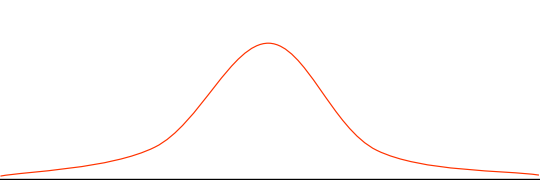
\includegraphics[width=.6\textwidth]{img/H.png}
		\end{center}
		\item G: discrete, with mass at $\phi_k$
		\begin{center}
			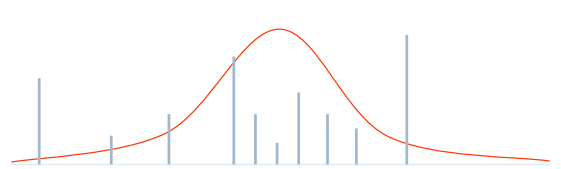
\includegraphics[width=.6\textwidth]{img/G.png}
		\end{center}
	\end{itemize}
\end{frame}

\begin{frame}
	\frametitle{An Alternative View of Gaussian Mixture}
	\begin{itemize}
		\item Recall
		\[
			G = \sum_{k=1}^{K}\pi_k\delta_{\phi_k}
		\]
		\item Take $K \rightarrow \infty$,
		\[
			G = \sum_{k=1}^{\infty}\pi_k\delta_{\phi_k}
		\]
		\item To execute Bayesian inference, we have to find a prior for $G$
		\item Dirichlet Process
	\end{itemize}
\end{frame}

\begin{frame}
	\frametitle{Warmup: Dirichlet Distribution}
	\begin{itemize}
		\item Dirichlet distribution is defined over $K$-dimensional probility simplex
		\[
		\Omega_K=\{(\pi_1,\ldots,\pi_K): \pi_k\ge 0,\sum_k \pi_k =1 \}
		\]
		\item We say $(\pi_1,\ldots,\pi_K)$ is Dirichlet distributed with parameters $(\alpha_1, \ldots, \alpha_K)$, if
		\[
		p(\pi_1,\ldots,\pi_K)=\frac{\Gamma(\sum_k \alpha_k)}{\prod_k \Gamma(\alpha_k)}\prod_k \pi_k^{\alpha_k-1}
		\]
	\end{itemize}
\end{frame}

\begin{frame}
	\frametitle{Warmup: Dirichlet Distribution}
	\begin{itemize}
		\item {Aggregation Property:}
		If \[
			(\pi_1,\ldots,\pi_i, \pi_{i+1},\ldots, \pi_K) \sim \text{Dirichlet}(\alpha_1,\ldots,\alpha_i, \alpha_{i+1}, \ldots, \pi_k) 
		\]
		Then
		\[
		(\pi_1,\ldots,\pi_i+\pi_{i+1},\ldots, \pi_K) \sim \text{Dirichlet}(\alpha_1,\ldots,\alpha_i+ \alpha_{i+1}, \ldots, \pi_k) 
		\]
	\end{itemize}
\end{frame}

\begin{frame}
	\frametitle{Warmup: Dirichlet Distribution}
	\begin{itemize}
		\item {Converse of Aggregation Property:}	If 
		\begin{align*}
		(\pi_1,\dots, \pi_k) & \sim \text{Dirichlet}(\alpha_1, \ldots, \pi_K) \\
		t & \sim \text{Beta}(\alpha_i \beta, \alpha_i (1-\beta)) \\
		(aka (t, 1-t) &\sim \text{Dirichlet}(\beta\alpha_i , (1-\beta)\alpha_i ))
		\end{align*}
		Then
		\begin{align*}
		& (\pi_1,\ldots,t\pi_i,(1-t)\pi_i\ldots, \pi_K) \\
		& \sim \text{Dirichlet}(\alpha_1,\ldots,\beta\alpha_i, (1-\beta)\alpha_{i+1}, \ldots, \alpha_K) 
		\end{align*}
	\end{itemize}
\end{frame}
\begin{frame}
	\frametitle{Warmup: Dirichlet Distribution}
	\begin{itemize}
		\item {Dirichlet-Multinomial conjugacy:}	If 
		\begin{align*}
		(\pi_1,\dots, \pi_K) & \sim \text{Dirichlet}(\alpha_1, \ldots, \pi_K) \\
		z & \sim Multinomial(\pi_1,\dots, \pi_K) \\
		\end{align*}
		Then
		\[
		(\pi_1,\dots, \pi_k)|z \sim \text{Dirichlet}(\alpha_1+\delta_z(1), \ldots, \pi_K+\delta_z(K))
		\]
	\end{itemize}
\end{frame}

\subsection{Definition}
\begin{frame}
	\frametitle{Dirichlet Process}
	\begin{itemize}
		\item Starting from $\pi$, slice the space finer and finer, what do we get?
		\begin{align*}
			(\pi) & \sim Dirichlet(\alpha) \\
			(\pi_1, \pi_2) & \sim Dirichlet(\alpha_1, \alpha_2) \\
			(\pi_{11},\pi_{12}, \pi_{21}, \pi_{22}) & \sim Dirichlet(\alpha_{11},\alpha_{12}, \alpha_{21},\alpha_{22}) \ldots 
		\end{align*}
		\item Because the dividing schema is arbitrary, finnally, any finite partition of $\pi$ should follow Dirichlet distribution.
	\end{itemize}
\end{frame}

\begin{frame}
	\frametitle{Dirichlet Process}
	\begin{itemize}
		\item Let $G$ be a probability measure over $\Omega$. For any mesearable subset $A\subset \Omega$, $G(A)=p(x\in A), x\in \Omega$
		\item Dirichlet process (DP) is a distribution over $G$. 
		\item We write 
		\[
			G \sim \text{DP}(\alpha, H)
		\]
		if for any finite partition $(A_1, \ldots, A_n)$ of $\Omega$,
		\[
			(G(A_1), \ldots, G(A_n)) \sim \text{Dirichlet}(\alpha H(A_1), \ldots, \alpha H(A_n))
		\]
		\item $H$ is the {\color{red} base distribution}
		\[
		\text{E}(G(A)) = H(A)
		\]
		\item $\alpha$ is the {\color{red} concentration parameter}
		\[
		\text{Var}(G(A)) = \frac{H(A)(1-H(A))}{\alpha+1}
		\]
	\end{itemize}
\end{frame}

\begin{frame}
	\frametitle{Posterior Dirichlet Process}

\end{frame}

\begin{frame}
	\frametitle{Dirichlet Process}
	\begin{itemize}
		\item{Why is DP useful for clustering?}
		\item{Our definition is all about properties of DP. How to construct a concrete DP?}

	\end{itemize}
\end{frame}




\begin{frame}
	\frametitle{Posterior Dirichlet Process}

\end{frame}

\begin{frame}
	\frametitle{Posterior Dirichlet Process}
	\begin{itemize}
		\item Luckily, the posterior is easy to calculate
		\item Using dirichlet-multinomial conjugacy. For any partition $(A_1, \ldots, A_n)$,
		\[
		(G(A_1), \ldots, G(A_n))|\theta \sim \text{Dirichlet}(\alpha H(A_1)+\delta_{\theta}(A_1), \ldots, \alpha H(A_n)+\delta_{\theta}(A_1))
		\]
		where $\delta_{\theta}(A)=1$ iff. $\theta \in A$
		\item So 
			\[
			G|\theta \sim DP(\alpha+1, \frac{\alpha H + \delta_{\theta}}{\alpha+1})
			\]
		\item We will construct a DP based on the posterior.
	\end{itemize}
\end{frame}

\subsection{Stick Breaking Construction}
\begin{frame}
	\frametitle{Stick Breaking Construction}
	\begin{itemize}
		\item { Consider partition $(\theta_1, \Omega - \{\theta_1\}) $}
		\[
			(G(\theta_1), G(\Omega - \{\theta_1\}))|\theta_1 \sim \text{Dir}(\alpha H(\theta_1)+1, \alpha H(\Omega - \{\theta_1\}))
		\]
		\item Note that $G(A_2) = 1-G(A_1)$, $H(\theta)=0$, $H(\Omega)=1$
		\[
			G(\theta_1) \sim \text{Beta}(1, \alpha)
		\]
		\item Let $\beta_1 = G(\theta_1)$
		\[
			G = \beta_1 \delta_{\theta_1} + (1-\beta_1)G_1
		\]
		where $G_1$ is a renomalized probability measure on $\Omega - \{\theta_1\}$
	\end{itemize}
\end{frame}
\begin{frame}
	\frametitle{Stick Breaking Construction}
	\begin{itemize}
		\item {Continue the process}
		\begin{align*}
			G & =\beta_1 \delta_{\theta_1} + (1-\beta_1)G_1 \\
			G & =\beta_1 \delta_{\theta_1} + (1-\beta_1)(\beta_2 + (1-\beta_2)G_2) \\
			& \vdots \\
			G &= \sum_{k=1}^{\infty} \pi_k \delta_{\theta_k}
		\end{align*}
		where 
		\begin{align*}
		\beta_k & \sim \text{Beta}(1, \alpha) \\
		\pi_k & = \beta_k \prod_{i=1}^{k-1} (1-\beta_i) \qquad (\text{denoted by } \pi \sim \text{GEM}(\alpha))\\
		\theta_k & \sim H
		\end{align*}
		\item This is the stick breaking construction
	\end{itemize}
\end{frame}

\begin{frame}
	\frametitle{Stick Breaking Construction}
	\begin{itemize}
		\item What can we find about DP from this construction?
		\begin{itemize}
		\item A sample $G$ from DP is discrete with probability 1
		\item If we keep sampling from $G$, we'll get more and more repeated values
		\item That's what we need for clustering		
		\end{itemize}
	\end{itemize}
\end{frame}

\subsection{Blackwell-MacQueen Urn Scheme}
\begin{frame}
\frametitle{Blackwell-MacQueen Urn Scheme}
	\begin{itemize}
		\item{But for clustering, we're actually interested sampling mixture parameters $\theta_1, \theta_2, \ldots$ from $\Omega$, integrating $G$ out.}
		\item It seems easy. $\theta_1, \theta_2, \ldots, \theta_n$ are independent given G. So we can simply sample each $\theta$ from $H$ independently, right?
		\item No! $\theta$s are no longer indenpendent if we integrate $G$ out
		\[
		p(\theta_1, \theta_2, \ldots, \theta_n) = \int_G \prod_{i=1}^{n} p(\theta_i|G)p(G) \diff G
		\]
	\end{itemize}
\end{frame}
\begin{frame}
	\frametitle{Blackwell-MacQueen Urn Scheme}
	\begin{itemize}
		\item Consider two samples $\theta_1, \theta_2$.
		\begin{align*}
		p(\theta_2 | \theta_1) & = \int_G \prod_{i=1}^{n} p(\theta_2, G| \theta_1) \diff G \\
		& = \int_G \prod_{i=1}^{n} p(\theta_2|G) p(G|\theta_1) \diff G 
		\end{align*}
		\item We have already known the distribution of $G$ given $\theta_1$,
		
		\[
		G|\theta_1 \sim \text{DP}(\alpha+1, \frac{\alpha H + \delta_{\theta_1}}{\alpha+1})
		\]
		\item Then, given $\theta_1$, the second sample $\theta_2$ can be sampled from the posterior base distribution.
		\item The sampling process becomes quite simple		
	\end{itemize}
\end{frame}
\begin{frame}
	\frametitle{Blackwell-MacQueen Urn Scheme}
	\begin{itemize}
		\item First sample: 
			\[ \theta_1 \sim H, \quad G|\theta_1 \sim \text{DP}(\alpha+1, \frac{\alpha H + \delta_{\theta_1}}{\alpha+1}) \]
		\item Second sample:
			\[ \theta_2|\theta_1 \sim \frac{\alpha H + \delta_{\theta_1}}{\alpha+1}, \quad G|\theta_1,\theta_2 \sim \text{DP}(\alpha+2, \frac{\alpha H + \delta_{\theta_1} + \delta_{\theta_2}}{\alpha+2}) \]
		\item $n^{th}$ sample:
			\[ \theta_n|\theta_{1,\ldots,n-1} \sim \frac{\alpha H + \sum_{k=1}^{n-1}\delta_{\theta_k}}{\alpha+n-1}, \quad G|\theta_{1,\ldots,n} \sim \text{DP}(\alpha+n, \frac{\alpha H + \sum_{k=1}^{n}\delta_{\theta_k}}{\alpha+n}) \]
	\end{itemize}
\end{frame}

\begin{frame}
	\frametitle{Blackwell-MacQueen Urn Scheme}
	\begin{itemize}
		\item One issue, how to sample from $\frac{\alpha H + \sum_{k=1}^{n-1}\delta_{\theta_k}}{\alpha+n-1}$?
		\begin{itemize}
			\item With probability $\propto \alpha$, sample from $H$
			\item With probability $\propto n-1$, randomly pick one from $\theta_1,\ldots,
			 \theta_{n-1}$
		\end{itemize}
		\item The above sample process is called {\em Blackwell-MacQueen Urn Scheme}
		\item Working with float value is annoying. Can we
	\end{itemize}
\end{frame}

\begin{frame}
\frametitle{Chinese Restaurant Process(CPR)}
\end{frame}


\begin{frame}
\frametitle{Stick Breaking Consturction}
\end{frame}


\end{document}